\documentclass{article}

\usepackage{graphicx}
\usepackage{tikz}
\usepackage{tikzsymbols}
\usetikzlibrary{calc,patterns,shapes.geometric}
\pagestyle{empty}
\usepackage[margin=0pt]{geometry}
\geometry{papersize={14in,12in}}

\def\centerarc[#1](#2)(#3:#4:#5){\draw[#1] ($(#2)+({#5*cos(#3)},{#5*sin(#3)})$) arc (#3:#4:#5);}

\begin{document}
	\begin{figure}
		\centering
		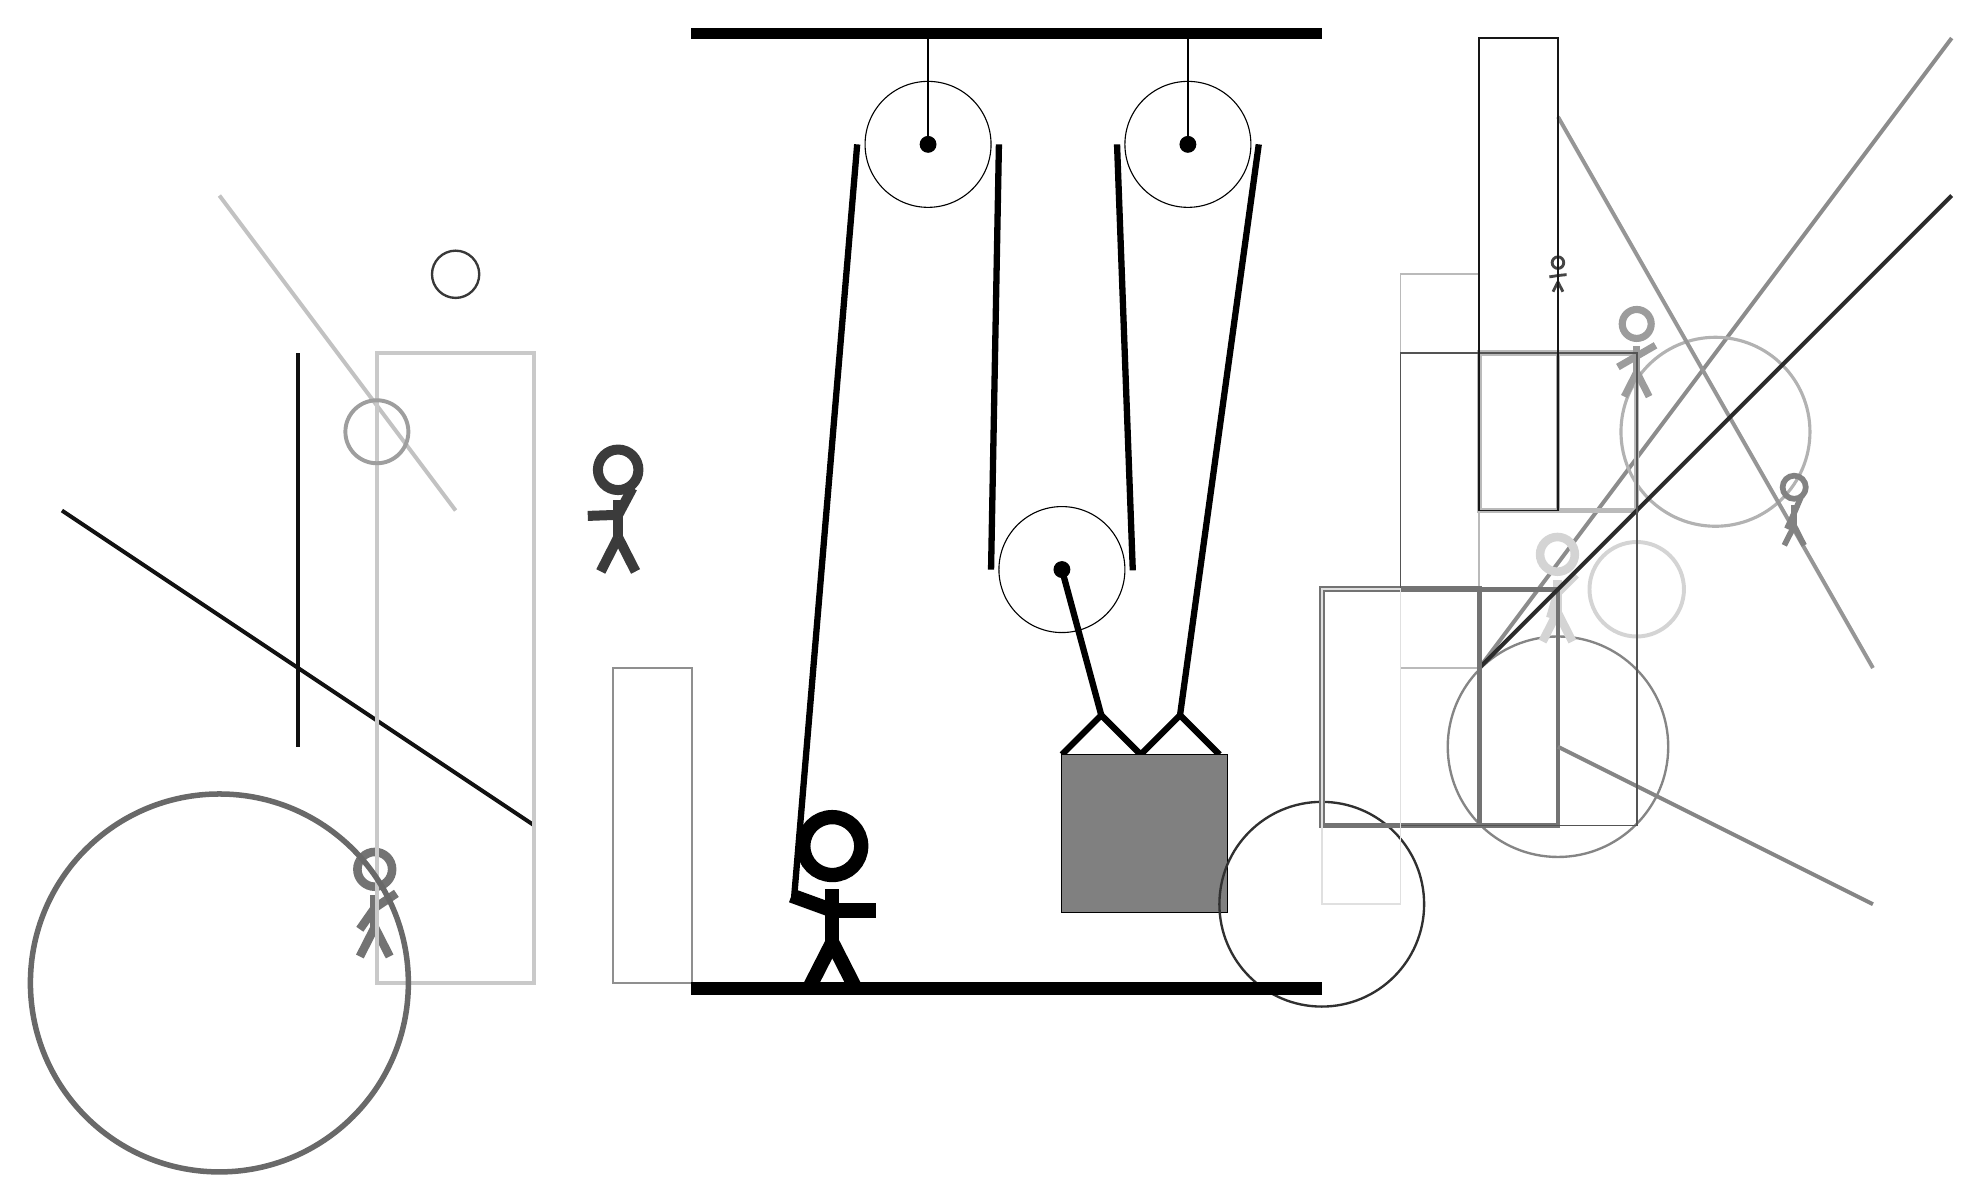
\begin{tikzpicture}
			%%%%% START %%%%%
			
			\draw[fill=black] (-2, 9) rectangle (6, 9.125);
			
			\draw (1, 7.65) circle (0.8);
			\draw[fill=black] (1, 7.65) circle (0.1);
			\draw[thick] (1, 7.65) -- (1, 9);
			
			\draw (4.3, 7.65) circle (0.8);
			\draw[fill=black] (4.3, 7.65) circle (0.1);
			\draw[thick] (4.3, 7.65) -- (4.3, 9);
			
			\draw (2.7, 2.25) circle (0.8);
			\draw[fill=black] (2.7, 2.25) circle (0.1);
			
			\draw[line width=0.8mm]  (2.7, -0.1) -- (3.2, 0.4) -- (3.7, -0.1) -- (4.2, 0.4) -- (4.7, -0.1);
			\draw[fill=black!50] (2.7, -0.1) rectangle (4.8, -2.1);
			
			\draw[line width=0.8mm](-0.7, -1.9) -- (0.1, 7.65);
			\centerarc[line width=0.8mm](1, 7.65)(0:180:0.9);
			\draw[line width=0.8mm](1.9, 7.65) -- (1.8, 2.25);
			\centerarc[line width=0.8mm](2.7, 2.25)(180:370:0.9);
			\draw[line width=0.8mm] (3.6, 2.24) -- (3.4, 7.65);
			\centerarc[line width=0.8mm](4.3, 7.65)(0:180:0.9);
			\draw[line width=0.8mm](4.2, 0.4) -- (5.2, 7.65);
			\draw[line width=0.8mm] (3.2, 0.4) -- (2.7, 2.25);
			
			\draw[line width=0.5mm, color=black!93](-4, -1) -- (-10, 3);
			
			\draw[line width=0.5mm, color=black!45](8, 1) -- (14, 9);
			\node[line width=0.2mm, color=black!55] at (-6, -2) {\Strichmaxerl[6][55][34]};
			\draw [line width=0.3mm, color=black!48](9, 0) circle (1.4);
			\draw [line width=0.4mm, color=black!30](11, 4) circle (1.2);
			\draw[line width=0.2mm, color=black!27] (7, 1) rectangle (8, 6);
			
			\draw [line width=0.3mm, color=black!78](-5, 6) circle (0.3);
			\node[line width=0.7mm, color=black!17] at (9, 2) {\Strichmaxerl[6][74][45]};
			\draw[line width=0.7mm, color=black!27] (8, 5) rectangle (10, 3);
			\draw [line width=0.3mm, color=black!81](6, -2) circle (1.3);
			\draw[line width=0.5mm, color=black!41](9, 8) -- (13, 1);
			\draw [line width=0.5mm, color=black!17](10, 2) circle (0.6);
			\draw[line width=0.5mm, color=black!33](9, 5) -- (9, 3);
			
			\draw[line width=0.5mm, color=black!94](-7, 5) -- (-7, 0);
			\draw[line width=0.6mm, color=black!55] (6, 2) rectangle (9, -1);
			\draw[line width=0.2mm, color=black!44] (-3, 1) rectangle (-2, -3);
			
			\draw[line width=0.5mm, color=black!83](8, 1) -- (14, 7);
			\node[line width=0.7mm, color=black!39] at (10, 5) {\Strichmaxerl[5][30][30]};
			\node[line width=0.2mm, color=black!49] at (12, 3) {\Strichmaxerl[4][65][67]};
			\draw [line width=0.3mm, color=black!73](6, 6) circle (0.0);
			\draw[line width=0.5mm, color=black!48](9, 0) -- (13, -2);
			
			\draw[line width=0.7mm, color=black!55] (6, 2) rectangle (8, -1);
			
			\draw[line width=0.5mm, color=black!24](-5, 3) -- (-8, 7);
			\node[line width=0.5mm, color=black!73] at (9, 6) {\Strichmaxerl[2][9][6]};
			\node[line width=0.2mm, color=black!77] at (-3, 3) {\Strichmaxerl[7][2][62]};
			
			\draw[line width=0.5mm, color=black!21] (-4, 5) rectangle (-6, -3);
			
			\draw[line width=0.2mm, color=black!67] (7, 5) rectangle (10, -1);
			\draw [line width=0.5mm, color=black!38](-6, 4) circle (0.4);
			
			\draw[line width=0.2mm, color=black!12] (7, -2) rectangle (6, 2);
			
			\draw [line width=0.7mm, color=black!59](-8, -3) circle (2.4);
			\draw[line width=0.2mm, color=black!91] (8, 3) rectangle (9, 9);
			
			
			\node at (-0.2, -2) {\Strichmaxerl[10][-20][0]};
			
			\draw[fill=black] (-2, -3) rectangle (6, -3.15);
			
			%%%%% END %%%%%
		\end{tikzpicture}
	\end{figure}	
\end{document}